\subsubsection{K-联通块}
N个点的树,点上有权值,求大小为K的联通块权值和的最大值。$K\le N\le 100.$

$f[i,j]$表示以$i$为根(包括$i$点),大小为$j$的联通块的权值和。
\begin{equation*}
    f[i,j]=\max\left\{\sum_{p=1}^kdp[ik,jp]\right\}+v_i
\end{equation*}

转换成背包?有依赖的背包问题+泛化物品。假设现在有$j-1$块钱,对于每个孩子可以选择选和不选,选则增加收益,现在要求最大化收益。

所以本质上还是一个背包问题。要对背包问题形成敏感性,看到以上式子就应该考虑树上背包问题。
\begin{figure}[h]
    \begin{center}
        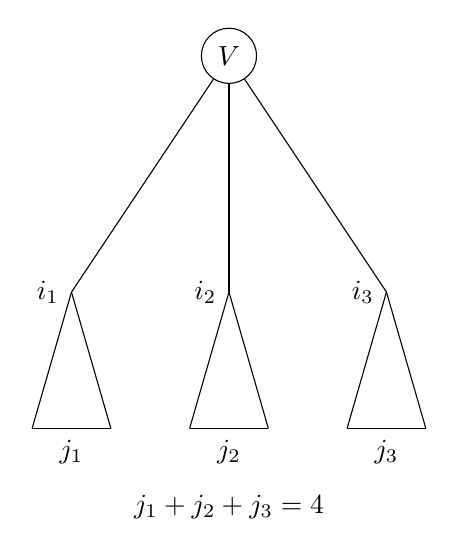
\begin{tikzpicture}
            [Node/.style={circle,draw=black,thin,radius=5mm}];
            \node[Node] (v) at (0,4.732) {$V$};

            \draw (-2,1.732)--(-1.5,0);
            \draw (-2.5,0)--(-1.5,0);
            \draw (-2.5,0)--(-2,1.732);
            \draw (v) to (-2,1.732);

            \draw (-0.5,0)--(0.5,0);
            \draw (-0.5,0)--(0,1.732);
            \draw (0.5,0)--(0,1.732);
            \draw (v) to (0,1.732);

            \draw (2.5,0)--(1.5,0);
            \draw (2.5,0)--(2,1.732);
            \draw (1.5,0)--(2,1.732);
            \draw (v) to (2,1.732);

            \node at (-2,-0.3) {$j_1$};
            \node at (0,-0.3) {$j_2$};
            \node at (2,-0.3) {$j_3$};

            \node at (-2.3,1.732) {$i_1$};
            \node at (-0.3,1.732) {$i_2$};
            \node at (1.7,1.732) {$i_3$};

            \node at (0,-1) {$j_1+j_2+j_3=4$};
        \end{tikzpicture}
    \end{center}
    \caption{对状态转移的解释:图中$i_k$表示枚举子树的编号为$k$,$j_p$表示分配给这棵子树的大小为$p$。}
    \label{fig. 1.1}
\end{figure}
\subsection{状态压缩模型}
\subsubsection{棋盘上的王}
定义$dp[i,j,s]$表示前$i$行已经放了$j$个,并且前$i$行已经在$s$的集合中放了王。枚举集合$s'$为倒数第二行放的状态,且s与$s'$不互相攻击。
\begin{equation*}
    \begin{aligned}
        dp[i,j,s]=&\sum_{s'}dp[i,j-|s|,s']\\
        dp[i,j,s]\to& dp[i,j+|s|,s']
    \end{aligned}
\end{equation*}
状态压缩实际上是表示状态的一种技巧,可以将集合$s$转化成一个长度为$n$的01字符串,共有$2^n-1$中取值(状态压缩中的“压缩”对应将集合转化为一个数字)。

\begin{minted}{C++}
#include<cstdlib>
#include<cstring>
#include<cmath>
#include<cstdio>

const int Modulo = int(1e9+7);

void update(int &a,int &b) {
    a=(a % Modulo + b % Modulo) % Modulo;
}

int pop_count(int S) {
    int ans = 0;
    while(S) {
        if(S & 1) ans++;
        S >>= 1;
    }
    return ans;
}

bool is_valid(int S) {
    return ! bool(S & (S >> 1));
}

bool is_valid2(int S1,int S2) {
    return ! (bool(S1 & S2) || bool(S1 & (S2 >> 1)) || bool(S1 & (S2 << 1)));
}

int n,k,dp[11][101][1024];

int main(void) {
    scanf("%d%d", &n, &k);

    dp[0][0][0] = 1;
    for(int i = 1; i <= n; ++i) {
        for(int j = 0; j <= k; ++j) {
            for(int S = 0; S < (1 << n); ++S) if(is_valid(S)&&pop_count(S)<=j) {
                for(int SS = 0; SS < (1 << n); ++SS) if(is_valid(SS)) {
                    if(is_valid2(S, SS)) {
                        update(dp[i][j][S], dp[i-1][j-pop_count(S)][SS]);
                    }
                }
            }
        }
    }

    int ans = 0;
    for(int S = 0; S < (1 << n); ++S) if(is_valid(S)) {
            update(ans,dp[n][k][S]);
    }

    printf("%d",ans);
    return 0;
}
\end{minted}

\subsubsection{联通}
N个点,M条边,要求选一些边,使得给定4对点分别联通,求最小的边权和。$N\le 30, M\le 1000.$
\begin{figure}[h]
    \begin{center}
        \begin{tikzpicture}
            [Node/.style={circle,draw=black,thin,radius=5mm}];
            \node[Node] (c1) at (0,2) {$\ $};
            \node[Node] (c2) at (0,-2) {$\ $};
            \node[Node] (l1) at (-2,3) {$\ $};
            \node[Node] (l2) at (-2,-3) {$\ $};
            \node[Node] (r1) at (2,3) {$\ $};
            \node[Node] (r2) at (2,-3) {$\ $};
            \draw [thin,sloped,above] (c1) to node {$1.5$} (c2);
            \draw [thin,sloped,above] (c1) to node {$1$} (l1);
            \draw [thin,sloped,above] (c1) to node {$1$} (r1);
            \draw [thin,sloped,above] (c2) to node {$1$} (l2);
            \draw [thin,sloped,above] (c2) to node {$1$} (r2);
            \draw [thin] (r1)..controls(4,0)..(r2);
            \node (flag) at (3.75,0) {$3$};
            \draw [thin] (l1)..controls(-4,0)..(l2);
            \node (flag) at (-3.75,0) {$3$};
        \end{tikzpicture}
    \end{center}
    \caption{部分算法的反例,图中的最优解应为5.5.}
    \label{fig. 1.2}
\end{figure}

想想最后的答案如何构成,最后的答案一定是由几棵生成树组成。在图的连通性的状态压缩时,往往使用$dp[s]$表示使得集合$s$里的点两两联通的方案数。

类似于区间DP中的想法,我们把一个集合分为两个集合,把左半部分连接起来,然后再把右半部分连接起来,最后找一个中介把两个集合合并起来。我们可以把一部分点连接起来,然后再把另一部分点连起来,最后找一个“桥梁”把两部分连接起来。更一般地想,我们有两个联通块,那么我们需要找到两个根节点使得代价最小。

处理这类问题的常用技巧,加一维$i$,$f[i,s]$表示一定经过$i$这个点把$s$中的点两两联通所需的最小代价,状态表示以$i$为根形成的生成树的最小代价。
\begin{figure}[H]
    \begin{center}
        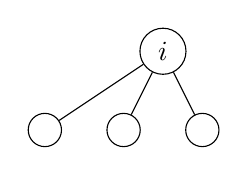
\begin{tikzpicture}
            [Node/.style={circle,draw=black,thin,radius=5mm}];
            \node[Node] (root) at (0.5,1){$i$};
            \node[Node] (n1) at (-1,0){$\ $};
            \node[Node] (n2) at (0,0){$\ $};
            \node[Node] (n3) at (1,0){$\ $};
            \draw[-](root) to (n1);
            \draw[-](root) to (n2);
            \draw[-](root) to (n3);
        \end{tikzpicture}
    \end{center}
    \caption{如此设计状态的灵感}
    \label{fig. 1.3}
\end{figure}
\begin{equation*}
    \begin{aligned}
        f[i,s]=\min
        \begin{cases}
            \min\limits_{j}\{f[j,s]+dis[i,j]\},\\
            \min\limits_{s'\subseteq s}\{f[i,s']+f[i,s-s']\}.
        \end{cases}
    \end{aligned}
\end{equation*}
\begin{figure}[h]
    \begin{center}
        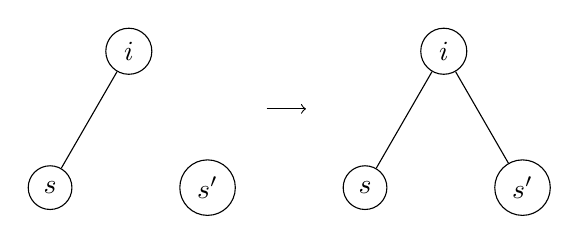
\begin{tikzpicture}
            [Node/.style={circle,draw=black,thin,radius=5mm}];
            \node[Node] (n1) at (-1, 0){$s$};
            \node[Node] (n2) at (1, 0){$s'$};
            \node[Node] (root) at (0,1.732){$i$};
    	    \draw [-](n1) to (root);
    	    \node[Node] (n1) at (3, 0){$s$};
            \node[Node] (n2) at (5, 0){$s'$};
            \node[Node] (root) at (4,1.732){$i$};
            \draw [-](n1) to (root);
    	    \draw [-](n2) to (root);
    	    \draw [->](1.75,1) to (2.25,1);
        \end{tikzpicture}
    \end{center}
    \caption{对状态转移的第二项的解释}
    \label{fig. 1.4}
\end{figure}

定义一个辅助数组$f^*[s]$表示枚举一个根节点后不管经过多少个点,把$s$集合内所有的点都联通所需要的最小代价。定义一个$g[s]$表示使得$s$这个集合中的点符合题目条件所需要的最小代价。$s$必须是一个合法的状态,即配对的两个点在里面,不能够成单的存在在$s$里。
\begin{equation*}
    \begin{aligned}
        f^*[s]=&\min\{f[s]\},\\
        g[s]=&\min\limits_{s^*\subseteq s}\{f^*[s^*]+g[s-s^*]\}.
    \end{aligned}
\end{equation*}
